\documentclass[aspectratio=169]{../latex_main/tntbeamer}  % you can pass all options of the beamer class, e.g., 'handout' or 'aspectratio=43'
\usepackage{dsfont}
\usepackage{bm}
\usepackage[english]{babel}
\usepackage[T1]{fontenc}
%\usepackage[utf8]{inputenc}
\usepackage{graphicx}
\graphicspath{ {./figures/} }
\usepackage{algorithm}
\usepackage[ruled,vlined,algo2e,linesnumbered]{algorithm2e}
\usepackage{hyperref}
\usepackage{booktabs}
\usepackage{mathtools}

\usepackage{amsmath,amssymb}

\DeclareMathOperator*{\argmax}{arg\,max}
\DeclareMathOperator*{\argmin}{arg\,min}

\usepackage{pgfplots}
\pgfplotsset{compat=1.16}
\usepackage{tikz}
\usetikzlibrary{trees} 
\usetikzlibrary{shapes.geometric}
\usetikzlibrary{positioning,shapes,shadows,arrows,calc,mindmap}
\usetikzlibrary{positioning,fadings,through}
\usetikzlibrary{decorations.pathreplacing}
\usetikzlibrary{intersections}
\pgfdeclarelayer{background}
\pgfdeclarelayer{foreground}
\pgfsetlayers{background,main,foreground}
\tikzstyle{activity}=[rectangle, draw=black, rounded corners, text centered, text width=8em]
\tikzstyle{data}=[rectangle, draw=black, text centered, text width=8em]
\tikzstyle{myarrow}=[->, thick, draw=black]

% Define the layers to draw the diagram
\pgfdeclarelayer{background}
\pgfdeclarelayer{foreground}
\pgfsetlayers{background,main,foreground}

% Requires XeLaTeX or LuaLaTeX
\usepackage{unicode-math}

\usepackage{fontspec}
%\setsansfont{Arial}
\setsansfont{RotisSansSerifStd}[ 
Path=../latex_main/fonts/,
Extension = .otf,
UprightFont = *-Regular,  % or *-Light
BoldFont = *-ExtraBold,  % or *-Bold
ItalicFont = *-Italic
]
\setmonofont{Cascadia Mono}[
Scale=0.8
]

% scale factor adapted; mathrm font added (Benjamin Spitschan @TNT, 2021-06-01)
%\setmathfont[Scale=1.05]{Libertinus Math}
%\setmathrm[Scale=1.05]{Libertinus Math}

% other available math fonts are (not exhaustive)
% Latin Modern Math
% XITS Math
% Libertinus Math
% Asana Math
% Fira Math
% TeX Gyre Pagella Math
% TeX Gyre Bonum Math
% TeX Gyre Schola Math
% TeX Gyre Termes Math

% Literature References
\newcommand{\lit}[2]{\href{#2}{\footnotesize\color{black!60}[#1]}}

%%% Beamer Customization
%----------------------------------------------------------------------
% (Don't) Show sections in frame header. Options: 'sections', 'sections light', empty
\setbeamertemplate{headline}{empty}

% Add header logo for normal frames
\setheaderimage{
	% 
\includegraphics[height=\logoheight]{figures/TNT_darkv4.pdf}
	
\includegraphics[height=\logoheight]{../latex_main/figures/luh_logo_rgb_0_80_155.pdf}
	% 
\includegraphics[height=\logoheight]{figures/logo_tntluh.pdf}
}

% Header logo for title page
\settitleheaderimage{
	% 
\includegraphics[height=\logoheight]{figures/TNT_darkv4.pdf}
	
\includegraphics[height=\logoheight]{../latex_main/figures/luh_logo_rgb_0_80_155.pdf}
	% 
\includegraphics[height=\logoheight]{figures/logo_tntluh.pdf}
}

% Title page: tntdefault 
\setbeamertemplate{title page}[tntdefault]  % or luhstyle
% Add optional title image here
%\addtitlepageimagedefault{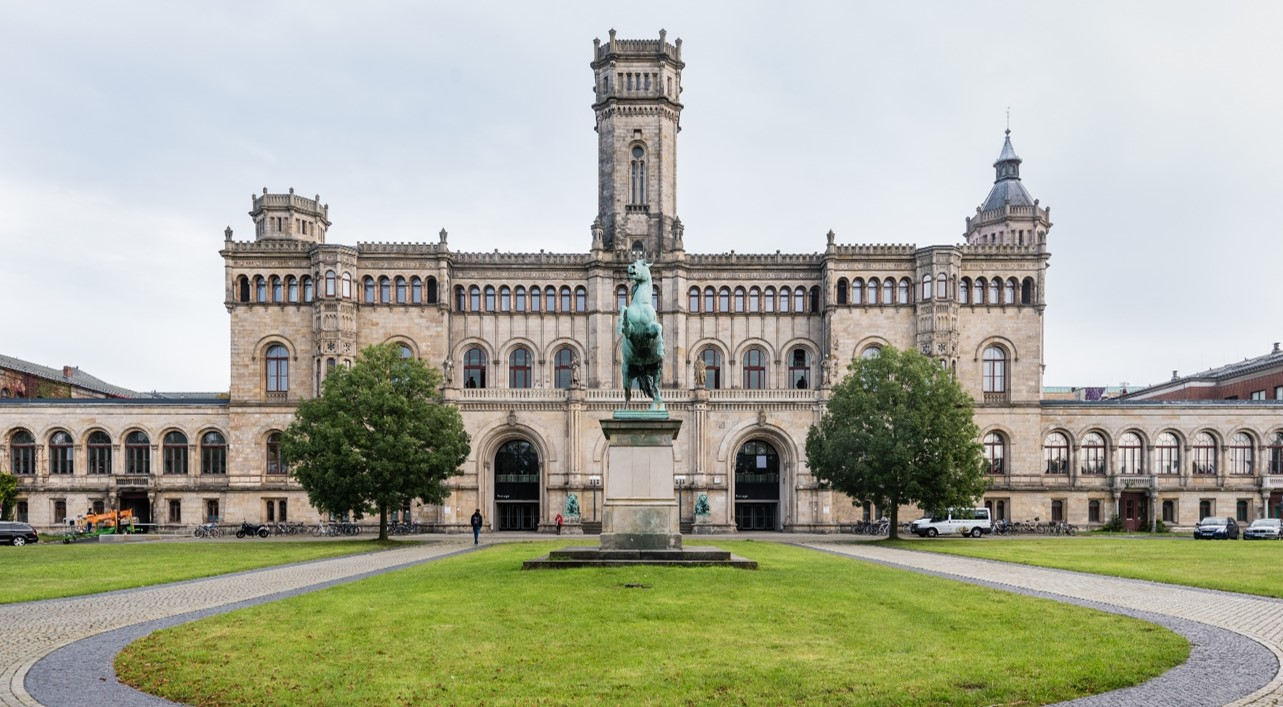
\includegraphics[width=0.65\textwidth]{figures/luh_default_presentation_title_image.jpg}}

% Title page: luhstyle
% \setbeamertemplate{title page}[luhstyle]
% % Add optional title image here
% \addtitlepageimage{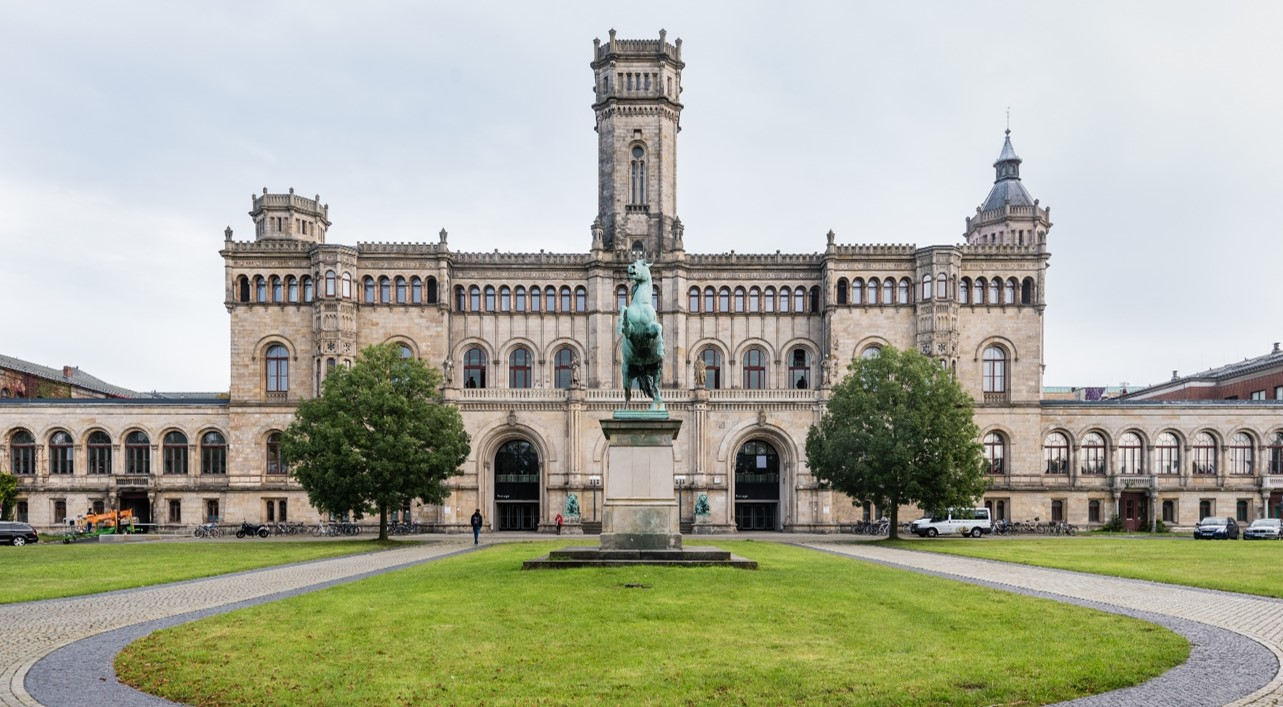
\includegraphics[width=0.75\textwidth]{figures/luh_default_presentation_title_image.jpg}}

\author[Lindauer \& Anand]{Marius Lindauer and Avishek Anand\\[1em]
	
\includegraphics[height=\logoheight]{../latex_main/figures/luh_logo_rgb_0_80_155.pdf}\qquad

\includegraphics[height=\logoheight]{../latex_main/figures/TNT_darkv4}\qquad

\includegraphics[height=\logoheight]{../latex_main/figures/L3S.jpg}	}
\date{Winter Term 2021
}


%%% Custom Packages
%----------------------------------------------------------------------
% Create dummy content
\usepackage{blindtext}

% Adds a frame with the current page layout. Just call \layout inside of a frame.
\usepackage{layout}


\title[Introduction]{iML: Introduction}
\subtitle{The Big Picture}

%\institute{}


\begin{document}
	
	\maketitle

	%-----------------------------------------------------------------------------------------------------------------------------

	\begin{frame}[c]{Why Interpretability?}
		
		\begin{itemize}
			\item Machine Learning (ML) has a huge potential to aid the decision-making process in various scientific and business applications due to its predictive power.
			\pause
			\smallskip
			\item ML models usually are intransparent black boxes, e.g., XGBoost, RBF SVM or DNNs.
			\begin{itemize}
				\item[$\leadsto$] too complex to be understood by humans
			\end{itemize}
			\pause
			\smallskip
			\item The lack of explanation
			\begin{enumerate}
				\item hurts trust
				\item creates barriers
			\end{enumerate}  
			\pause
			\smallskip
		    \item[$\leadsto$] Harder to adapt for critical areas with decisions affecting human life (e.g., medicine or credits).
			\pause
			%\smallskip
			\item[$\leadsto$] Many disciplines with required trust rely on traditional models,\\ e.g., linear models, with less predictive performance.
		\end{itemize}
		
	\end{frame}
	
	%-----------------------------------------------------------------------------------------------------------------------------	
	
	\begin{frame}[c]{Brief History of Interpretability}
		\begin{itemize}
			\item 18th and 19th century: linear regression models (Gauss, Legendre, Quetelet)
			\item 1940s: sensitivity analysis (SA), still used today
			\item Middle of 20th century: Rule-based ML, incl. decision rules and decision trees
			\item 2001: built-in feature importance measure of random forests
			\item >2010: explainable AI (XAI) for deep learning
			\item >2015: IML as an independent field of research 
			\item 2018: GDPR requires explainability for some applications 
		\end{itemize}
	\end{frame}
	
	%-----------------------------------------------------------------------------------------------------------------------------
	
	\begin{frame}[c]{When do We Need Interpretability? \lit{Doshi-Velez and Kim. 2017}{https://arxiv.org/abs/1702.08608}
		\lit{Adadi and Adadi. 2018}{https://ieeexplore.ieee.org/document/8466590}}
		\begin{columns}
			\begin{column}{0.6\textwidth}
				\begin{itemize}
					\item To \textbf{Justify} (and increase trust in models): investigate if and why biased, unexpected or discriminatory predictions were made.
					\pause
					\item To \textbf{Control}: debug models, identify and correct vulnerabilities and flaws.
					\pause
					\item To \textbf{Improve}: understanding why a prediction was made makes it easier to improve the model.
					\pause
					\item To \textbf{Discover}: learn new facts, gather information and gain insights.
				\end{itemize}
			\end{column}
			\begin{column}{0.6\textwidth}  
				\begin{center}
					\begin{figure}
						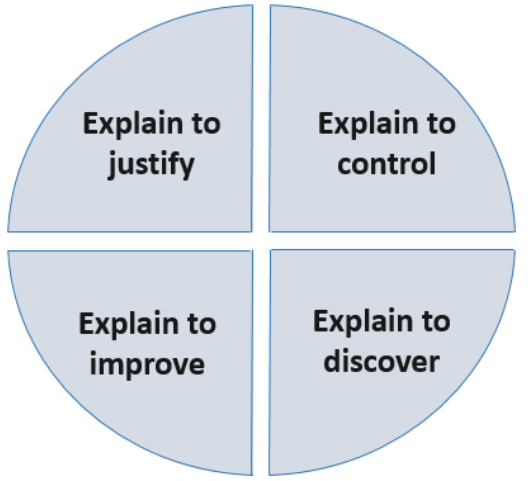
\includegraphics[width=0.58\textwidth]{figure/explain-to}
					\end{figure}
				\end{center}
			\end{column}
		\end{columns}

	\end{frame}
	
	%TODO: ADD who are stakeholder and what are high-stake scenarios
	
\end{document}
